
\subsection{Recording}
The structure of a recording is restrictive in terms of arranging the components due to the design of CESAR. There are numerous ways of presenting the recording view; however, a recording structure is limited to the components of starting a recording, establishing sensor connection, monitoring of samples, and finalize sensors and recording. Additional components can be incorporated to aid a recording without causing disruption. For instance, the connectivity state component (\ref{sssec:csc}) provides extended functionality to the recording structure. In Figure \ref{fig:hta_recording}, the illustration of a recording structure with the components and their dependencies are shown:

\begin{figure}
    \centering
    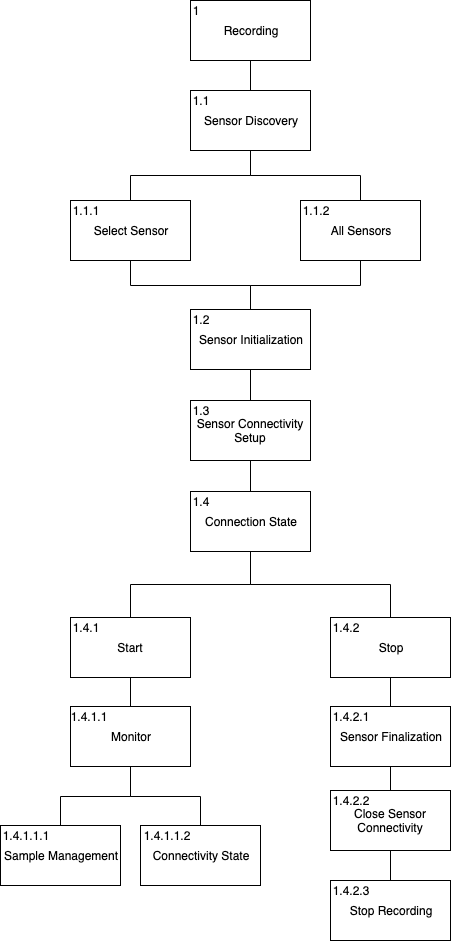
\includegraphics[scale=0.5]{images/Recording.png}
    \caption{Recording}
    \label{fig:hta_recording}
\end{figure}

\begin{itemize}
    \item[1.1] \verb|Sensor Discover:| Find all eligible sensors that can enable a recording.
    \item[1.1.1] \verb|Select Sensors:| From the sensor discovery, we can choose preferable sensors sources.
    \item[1.1.2] \verb|All Sensors:| more Straightforward, we sample from all of the available sensors.
    \item[1.2] \verb|Sensor Initialization:| Once we have a list of sensors sources, we need to establish and initialize a connection with the sensors. Occasionally a sensor might use some time to connect, or unforeseen occurrence is hindering the initialization of the sensor. Therefore, halting the sensor initalization or actively checking for sensor initalization is important. 
    \item[1.3] \verb|Sensor Connectivity Setup:| Establish a connection between the application and the sensor source through an API or IPC connection. All data exchange will occur over the established interface. 
    \item[1.4] \verb|Connection State:| Based on sensors establishments we can proceed to either start or stop a recording. 
    \item[1.4.1] \verb|Start:| By starting, we notify the sensors to begin collecting data, and the application should display that a recording has begun accordingly. Also, start a timer to display time elapsed on the current recording. 
    \item[1.4.1.1] \verb|Monitor:| Is a mechanism to handle the connectivty state and the incoming samples. It is actively listening to the interface for new data from the sensors, and appropriately distributing the data to the sample management component.  
    \item[1.4.1.1.1] \verb|Sample Management:| Handles a single sample from a sensor by parsing the content according to the payload of the sensor (each sensor might have different payload structure), such that it is according to our data structure.
    \item[1.4.1.1.2] \verb|Connectivity State:| Activly checking the state of sensor connectivty (read more below)
    \item[1.4.2] \verb|Stop:| Stop the recording timer and proceed to display results.
    \item[1.4.2.1] \verb|Sensor Finalization:| Notify the sensor to stop sampling data, and close establishment.
    \item[1.4.2.2] \verb|Close Sensor Connectivity:| Close the interface establishment between the application and the sensors. 
    \item[1.4.2.3] \verb|Stop Recording:| Once the sensors has closed its connections, add additional information to the recording (e.g., title, description, rating). In the end, the recording has concluded and it is stored on the mobile device.
\end{itemize}

\subsubsection{Connectivity State Component} \label{sssec:csc}
Connectivity state is a component that monitors for unexpected sensor disconnections or disruptions. Unexpected behavior can occur due to anomalies in the sensor, or the sensor being out of reach from the device for a brief moment.  A naive solution would be to ignore the connectivity state component, and assuming the sensors are connected to the device indefinitely. However, upon disconnections or disruptions, the recording would be missing samples which will result in a lacking record. This component solves the issue of missing samples by actively reconnecting the sensor based on a time interval, resulting in more accurate record with fewer gaps between samples. The following design questions for this component are 1) should the connectivity state component, which implements a time interval that tries to reconnect with the sensor, be implemented in the sensor wrapper, or should it be in the proposed recording structure?; and 2) should the interval between sample arrival be a fixed time or a dynamical time? 


\begin{enumerate}
    \item To achieve a mechanism of reconnecting to the sensor on unexpected disconnects or disruptions, establishing a time interval that monitors for sample arrivals within a time frame (e.g., every 10 seconds) is required. Incorporating the time interval in the sensor wrapper reduces the complexity of Nidra. However, it introduces extra complexity to the sensor wrappers. A sensor wrapper has to distinguish actual disconnects from unexpected disconnects. Although, by extending the functionality of sensor wrapper by implementing a state that indicates whether a recording is undergoing or stopped solves the problem. All future sensor wrappers would then have to implement the proposed solution, resulting in a complicated and time-consuming sensor wrappers development. While implementing the proposed solution in the sensor wrappers is possible, extending the recording structure with the logic in Nidra would be more meaningful and time-saving. In our design, we will be implementing the connectivity state in the recording structure.
    \item A time interval triggers an event every specified time frame. If an event is triggered, a sample has not arrived, meaning the sensor either has been disconnected or disrupted. A time frame can be in a fixed size (e.g., every 10 seconds) or a dynamical size (e.g., start with 10 seconds, then incrementally increase the frame by X seconds). Implementing a fixed time frame increases the stress on put on the sensor, whereas a dynamical time might miss samples if the time frame is significant. Depending on how critical the recording is, a suitable solution for the time frame should be configurable. Also, limiting the number of attempts made to reconnect should be considered, due to actively reconnecting to a sensor that is dead or completely out of reach can cause stress on the device. Thus, stopping the recording once a limited number of attempts has been reached.  In our design, we implemented a dynamical time and limited the number of attempts to 10. 
\end{enumerate}

\subsection{Sharing}

Sharing is separable into two concerns: export and import. The scope of exporting in Nidra is to select desired records, format and bundle the records into a transmittable file, and distributing the bundle over a media (e.g., mail). The scope of importing is to locate the file on the device, parse the content based on the format, and store it on the device. In Figure \ref{fig:hta_sharing}, the structure of sharing is presented with components and their dependencies: 

\begin{figure}
    \centering
    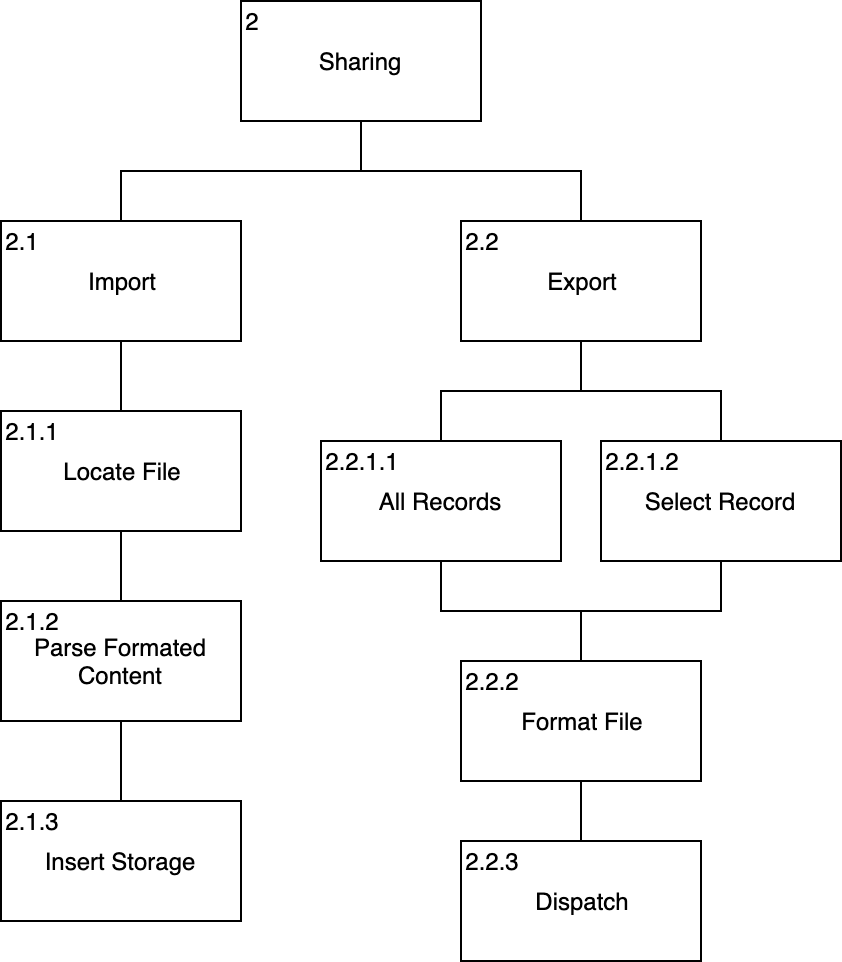
\includegraphics[scale=0.3]{images/Sharing.png}
    \caption{Sharing}
    \label{fig:hta_sharing}
\end{figure}

\begin{itemize}
    \item[2.1] \verb|Import|: Is a mechanism that locates a file, parse the data, and stores it on the device.
    \item[2.1.1] \verb|Locate File|: To enable this, the user has to download the file on the device. Then, locate the file on the device by using an interface to browse downloaded files. An interface can be developed; however, using the Android document picker (ref) is more straightforward solution.
    \item[2.1.2] \verb|Parse Formated Content|: Parse the content of the file accordingly to the data format (ref).
    \item[2.1.3] \verb|Insert Storage|: Retrieve the necessary data from the parsed file, to store on the device without overriding existing data.   
    \item[2.2] \verb|Export|: Is a mechanism that selects all or a specific record, format the record into a formatted filed (ref), and exports the file across device. 
    \item[2.2.1.1] \verb|All Records|: Export all of the records on the device.
    \item[2.2.1.2] \verb|Select Record|: Pick one specific record to export. 
    \item[2.2.2] \verb|Format File|: When a preferred format for the records is selected, bundling the data into a formatted file (ref) for transmittal can be done. It is essential to identify the name of the file uniquely to prevent duplicates and overrides of data. For instance, identifying the name of the file with the device identification appended with the time of exporting. 
    \item[2.2.3] \verb|Distribute|: Send the file across application (read more below).
\end{itemize}

\subsubsection{Distribute Component}
The distribute component uses the formatted file and transfers it across applications. There are two distinctive methods to perform this task which is efficient and practical: 1) implement an interface with recipients to share data with, by establish a web-server with logic to handle users and sharing data with the desired recipient. Also, implementing an interface to retrieve the file within the application;  and 2) using the interface provided by Android to share files. 

While the first option might be favorable in terms of practicality, this solution introduces additional concerns (e.g., the privacy matters of storing user data on a server) which is out of the scope for this project. For this reason, using the interface provided by Android is a reasonable solution. The user of the application can utilize the Android interface for sharing files over installed applications; however, e-mail is a flexible media to transfer the file, and the user can specify the recipients accordingly.  

\subsection{Modules}

\begin{figure}
    \centering
    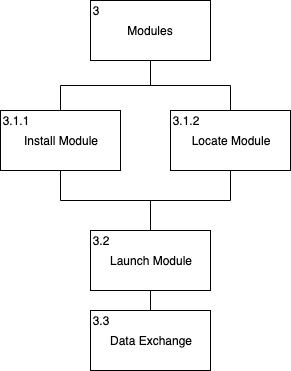
\includegraphics[scale=0.6]{images/Modules.png}
    \caption{Modules}
    \label{fig:hta_modules}
\end{figure}

Modules are independent applications that provide extended functionality and data enrichment to Nidra. The components for locating and launching a module is limited to Android design; however, the component for data exchange between a module and Nidra can be designed variously.  In Figure \ref{fig:hta_modules}, the structure of modules is presented with components and their dependencies:   

\begin{itemize}
    \item[3.1.1] \verb|Install Modules|: Is the process of locating the application on the device, and storing the reference of the application package name in the storage.  
    \item[3.1.2] \verb|Locate Module|: Retrieve the list of stored modules, and display the installed modules to the user. 
    \item[3.2] \verb|Launch Module|: Get the application location stored in the module, and launch the application with the use of Android Intent. 
    \item[3.3] \verb|Data Exchange|: Enrich the module with data from the application (read more below)
\end{itemize}

\subsubsection{Data Exchange Component}

The data exchange component facilitates the transportation of data between Nidra and a module. As of now, the data is records and corresponding samples, which is formatted (Section Data) accordingly. The two distinct methods to exchange data between a module and Nidra are 1) formatting all of the data and bundling it into the launch of the module, and 2) establishing a communication link for bi-directional requests between Nidra and the module. 

Android provides an interface to attach extra data on activity launch. The first solution is, therefore, convenient and efficient; all of the data is formatted and bundled into the launch. However, once Nidra has launched the module-application, there are no ways of transmitting new data besides relaunching the module-application. For this reason, the second option allows for continuous data flow by establishing a communication link with IPC between the applications. The data exchange between Nidra and modules can then be bidirectional; the module can request desired data any time, and Nidra can collect reports and results generated by the module. 

One could argue that new records are not obtained while managing and using a module. However, there might be future modules that do a real-time analysis of a recording, but that will require an interface for continuous data flow. For the simplicity of our design, we will be going with the first option of bundling all of the data and sending it on launch.

\subsection{Analytics}

\begin{figure}
    \centering
    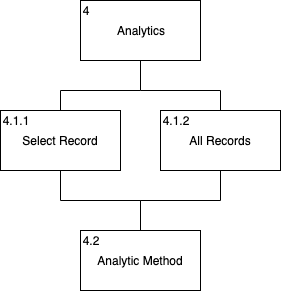
\includegraphics[scale=0.6]{images/Analytics.png}
    \caption{Analytics}
    \label{fig:hta_analytics}
\end{figure}

Analytics uses techniques and methods to gain valuable knowledge from data. Nidra provides a simple illustration of the data in a time-series plot; however, other techniques can be in incorporated. In essence, the facilitation of modules in the application enables the development opportunities for advanced analytics of the data. In Figure \ref{fig:hta_analytics}, the structure of analytics is presented with components and their dependencies: 

\begin{itemize}
    \item[4.1.1] \verb|Select Record|: locate the file on the device.
    \item[4.1.2] \verb|All Records|: parse the content of the file 
    \item[4.2] \verb|Analytic Method|: 
\end{itemize}

\subsubsection{Analytic Method Component}
The analytic method component uses the records on the device for representation or analysis. Graphical and non-graphical are two techniques for representing data. Graphical techniques visualize the data in a graph that enables analysis in various ways. A few graphical techniques are diagrams, charts, and time series. Non-graphical techniques, better known as statistical data tables, represent the data in tabular format. This provides a measurement of two or more values at a time \cite{datarepresentation}. More advanced techniques to analyze the data, are to use machine learning. Machine learning is concerned with developing data-driven algorithms, which can learn from observations without explicit instructions. For example, using recurrent neural networks (e.g., RNN, LSTM) or regression models (e.g., ARIMA), can be used to predict the sleeping patterns \cite{machinelearning}.

In Nidra, a time series graph is used to represent the data of a record. The time series graph represents the respiration data on the Y-axis and the time on the X-axis. Essentially, the facilitation of modules in the application is designed to enable advanced techniques to predict, analyze, and interpret the data acquisition. Therefore, in Nidra, the analytic methods are limited; however, the modules enable developers to construct any method they desire. 

\subsection{Storage}

\begin{figure}
    \centering
    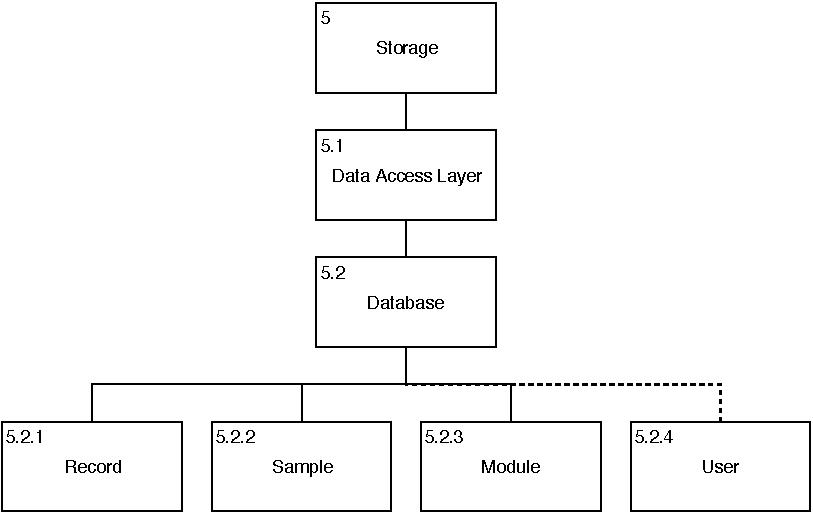
\includegraphics[scale=0.7]{images/Storage.pdf}
    \caption{Storage}
    \label{fig:hta_storage}
\end{figure}

Storage is the objective of achieving persistent data; data that is available after application termination. The data is characterized into four data entities (i.e., record, sample, module, and user) that contains individual properties.  The components in the storage structure are constructed to be extensible and scalable in terms of future data, restructure of data, and removal of data.  In Figure \ref{fig:hta_storage}, the structure of storage is presented with components and their dependencies: 

\begin{itemize}
    \item[5.1] \verb|Data Access Layer|: Also known as an Data Access Object (DAO), that provides an abstract interface to a database. It exposes spesific operations (such as insertion of a record) without revealing the database logic. The advantage of this interface is to have a single entry point for each database operation, and to easily extend and modify the operation for future data. 
    \item[5.2] \verb|Database|: Is the storage of all the data (read below).
    \item[5.2.1] \verb|Record|: Is a table in the database, which contains fields appropriately to the record structure. A record contains meta-data about a recording (e.g., name, recording time, user). The design decision and an example of a recording record is illustrated in (ref).
    \item[5.2.2] \verb|Sample|: Is a table in the database, which contains fields appropriately to a single sample from a sensor. A sample contains data received from a sensor during a recording. The design decision and an example of a sample record is illustrated in (ref).
    \item[5.2.3] \verb|Module|: Is a table in the database, which contains fields appropriately to the sample structure. A sample contains the name of the module and a reference to the application package. The design decision and an example of a module record is illustrated in (ref).
    \item[5.2.4] \verb|User|: Is an object stored on the device, which contains fields appropriately to the user structure. A user contains the patients biometrical information (e.g., name, weight, height). The design decision and an example of a user is illustrated in (ref).
\end{itemize}

\subsubsection{Database Component}

\noindent Android provides several options to store data on the device; depending on space requirement, type of data that needs to be stored, and whether the data should be private or accessible to other applications. Two suitable options for storage are 1) internal file storage - storing files to the internal storage private to the application; and 2) database - Android provides full support for SQLite databases, and the database access is private to the application \cite{android_storage}. Based on the options, some following design questions are 1) should the data be stored in a flat file database on the internal file storage, or should it be stored in an SQLite database?

Flat files database encode a database model (e.g., table) as a collection of records with no structured relationship, into a plain text or binary file. For instance, each line of text holds on a record of data, and the fields are separable by delimiters (e.g., comma or tabs). Another possibility is to encode the data in a preferable data format (ref formats). Flat file databases are easy to use and suited for small scale use; however, they provide no type of security, there is redundancy in the data, and integrity problems \cite{flatfilerdbms}. Locating a record is made possible by loading the file, and systematically iterating until the desired record is found. Similarly, updating a record and deleting a record. Consequently, the design of flat file databases is for simple and limited storage.

SQLite is a relational database management system, which is embedded and supported in Android. Relational database management system (RDBMS) provides data storage in fields and record, represented as columns (fields) and rows (records), in a table. The advantage is the ability to index records, relations between data stored in tables, and support querying of complex data with a query language (e.g., SQL). Also, RDBMS provides data integrity between transactions, improved security, and backup and recovery controls \cite{flatfilerdbms}. 

While a flat file database is applicable to store small and unchangeable data, it is not suitable for scalable and invasive data change. In Nidra, the samples acquisition makes it unreasonable to use a flat file database. Therefore, SQLite is a preferable solution to storing samples. Also, establishing a relationship between a record and a sample is made possible [rewrite]. 

\subsection{Presentation}
\begin{figure}
    \centering
    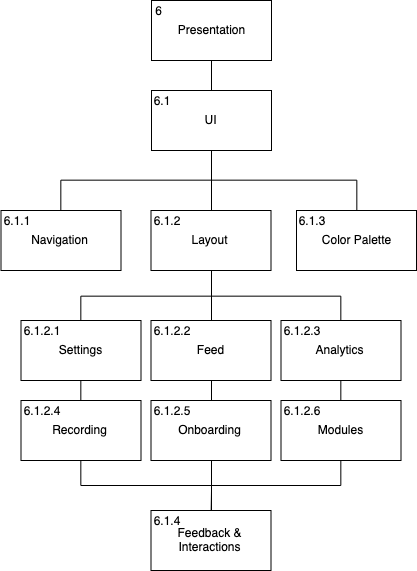
\includegraphics[scale=0.5]{images/Presentation.png}
    \caption{Presentation}
    \label{fig:hta_presentation}
\end{figure}

Presentation facilitates the user interface of the application, in terms of visualizing the functionality of the application to the user. The user interface derives from the functionality (concerns discussed) in the application, and research on the topic. In Figure \ref{fig:hta_presentation}, the structure of storage is presented with components and their dependencies: 

\begin{itemize}
    \item[6.1] \verb|UI|: The user interface where interaction between users and the application occurs. 
    \item[6.1.1] \verb|Layout|: Are the screen with the content of the current screen. The layout incorporates the color palette and some views have the navigation displayed. 
    \item[6.1.2] \verb|Navigation|: The navigation is a menu with options to change the layout. 
    \item[6.1.3] \verb|Color Palette|: A color selection that persist throughout the application (read more below).
    \item[6.1.1.1] \verb|Settings|: Is s screen with user details, permissions and credits, with options to modify permission and user details.
    \item[6.1.1.2] \verb|Feed|: Is a list of all records for the user, displayed with details specific to the record to make it distinguishable and easily recognizable. 
    \item[6.1.1.3] \verb|Analytics|: A interactive time-series graph for a single record. 
    \item[6.1.1.4] \verb|Recording|: The process of establishing a recording session, in addition to showing the results after a recording session has ended. 
    \item[6.1.1.5] \verb|Onboarding|: The initial screen displayed to the user, where the user can supply the application with their biometrical data. 
    \item[6.1.1.6] \verb|Modules|: A list of all installed modules, also an option to add more modules. 
    \item[6.1.4] \verb|Feedback & Interactions|: Each layout has different feedback and interaction, which should be handled appropriately. 
\end{itemize}

\subsubsection{Color Palette Component}
Color palette is a component that decides the color scheme in the application. In the proposal of a color system in the design guidelines by Google \cite{colorsystem}, it is essential to pick colors that reflect the style of the application accordingly to: 1) primary colors - the most frequently displayed color in the application; 2) secondary colors - provides an accent and distinguish color in the application; and 3) surface, background, error, typography and iconography colors - colors that reflect the primary and secondary color choices. 

Moreover, choosing colors that meet the purpose of the application is critical. Nidra is most likely to be used during the evening and the morning. According to Google \cite{darktheme}, a dark color theme reduces luminance emitted by the device screen, which reduces eye strain, while still meeting the minimum color contrast ratios, and conserving battery power. From this, we will be choosing a dark color theme. 